\section{Identyfikacja}


\subsection{Identyfikacja charakterystyki czujnika położenia}

Pomiar położenia sfery w układzie magnetycznej lewitacji jest dokonywany optycznie. Z jednej strony znajduje się źródło światła, a po przeciwnej stronie fotodioda z przetwornikiem A/C, która podaje pewne napięcie $u_x$. Podczas identyfikacji poszukujemy zależności tego napięcia od położenia sfery:

\begin{equation} \label{eq:gx}
u_x = g(x_1)
\end{equation}

Poszukujemy charakterystyki statycznej $g(x_1)$, którą otrzymamy przykręcając sferę do śruby i podnosząc ją co ustalony skok 0,7 mm. Za każdym razem dokonujemy pomiaru napięcia podanego przez detektor światła.

Do pracy z modelem potrzebna jest znajomość położenia sfery, dlatego na rysunku \ref{img:gx} charakterystyka odwrotną do zależności \ref{eq:gx}.

[trzeba przeskalować napięcie jeszcze, można zrobić wykres od -ux]

\begin{figure}[!htb]
\centering
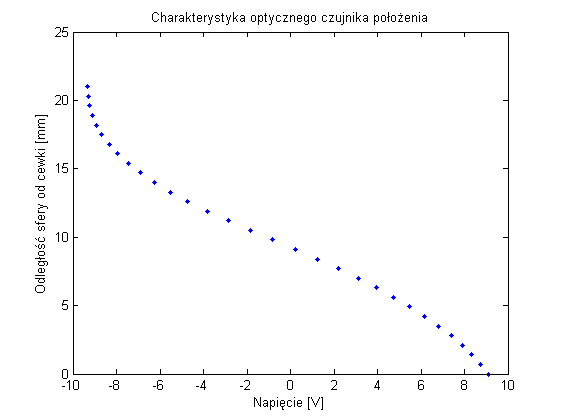
\includegraphics[scale=1]{img/czujnik_polozenia.png}
\caption{Charakterystyka statyczna optycznego czujnika położenia}
\label{img:gx}
\end{figure}


W pracy \cite{Bania1999} autor dokonał aproksymacji otrzymanej charakterystyki odwrotnej sumą funkcji wykładniczych metodą prób i błędów. Nie będziemy dokonywać takiej aproksymacji, ponieważ podczas pracy z modelem w laboratorium użyjemy bloku \textit{LUT z interpolacją} oferowanego przez Simulink.



\subsection{Identyfikacja parametrów cewki $k, T, u_c$ }

Aby wiedzieć, jak zmienia się prąd cewki w zależności od użytego sterowania, czyli przyłożonego napięcia $u$, należy wyznaczyć parametry $k, T$ oraz $u_c$.

\subsubsection{Pomiary w stanie ustalonym cewki}

Zależność prądu od napięcia jest liniowa
\begin{equation}
i = k(u + u_c)
\end{equation}

Parametry $k$ i $u_c$ (wzmocnienie oraz stałe napięcie na cewce) wyznaczymy mierząc prąd w stanie ustalonym dla różnych wartości napięcia sterującego.


\begin{figure}[!htb]
\centering
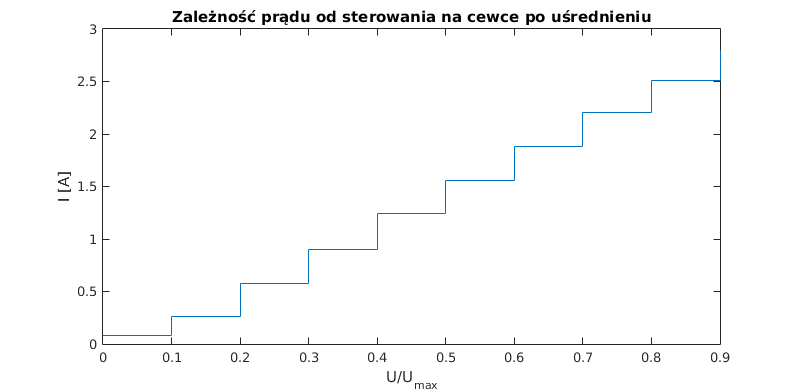
\includegraphics[scale=0.85]{img/prad_cewki_od_sterowania.png}
\caption{Identyfikacja parametrów statycznych cewki}
\label{rys:cewka_k_uc}
\end{figure}

\subsubsection{Pomiary stanów przejściowych cewki}

Stałą czasową cewki $T$ można wyznaczyć obserwując odpowiedź skokową prądu.
Zwalniamy PWM, zapinamy sterowanie (wypelnienie) na 50 procent i dzięki temu mamy skoki typowo napięciowe. Preskaler 4096.

\begin{figure}[H]
\centering
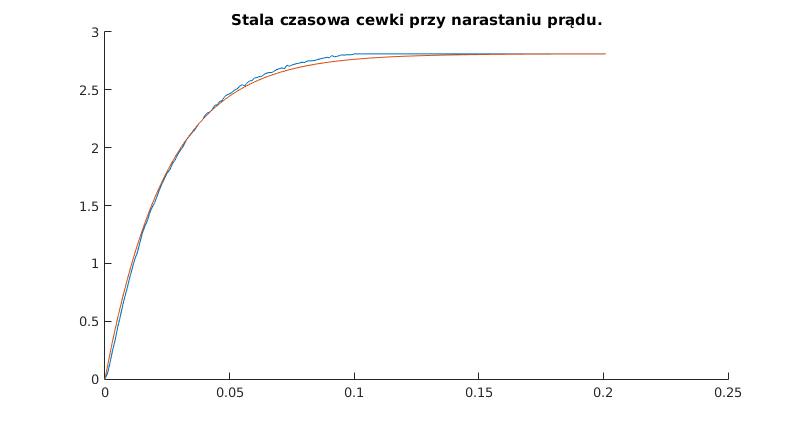
\includegraphics[scale=0.85]{img/identyfikacja_stala_narastanie_0245.png}
\caption{Identyfikacja parametrów statycznych cewki}
\label{rys:cewka_k_uc}
\end{figure}

\begin{figure}[H]
\centering
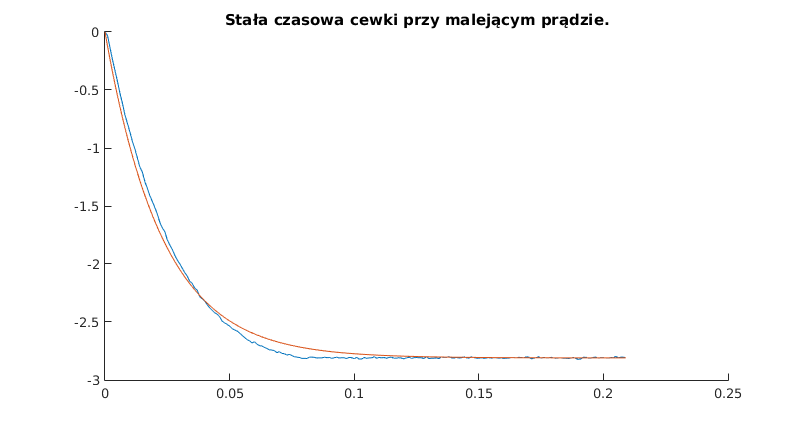
\includegraphics[scale=0.85]{img/identyfikacja_stala_opadanie_0230.png}
\caption{Identyfikacja parametrów statycznych cewki}
\label{rys:cewka_k_uc}
\end{figure}

%\begin{figure}[!ht]
%\centering
%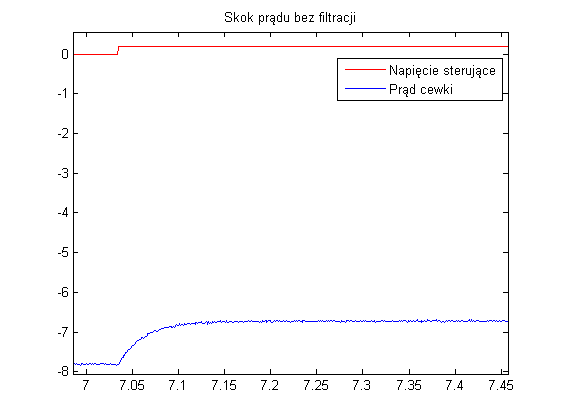
\includegraphics[scale=0.85]{img/skok_pradu_bezfiltra_pwm_szybkie.png}
%\caption{Identyfikacja stałej czasowej narastania prądu cewki [bez filtra, z PWM]}
%\label{rys:skok_pradu_bezfiltra}
%\end{figure}


Korzystając z metody najmniejszych kwadratów wyznaczono parametry, których wartości umieszczono w tabeli  \ref{tab:parametry_ident}.



\subsection{Identyfikacja indukcyjności cewki $L(x_1)$}

W celu identyfikacji zależności indukcyjności cewki od położenia w układzie otwartym należy wykonać serię pomiarów napięcia i prądu dla różnych położeń sfery. Zmierzona rezystancja cewki wynosi $R = 4,7\Omega$. Indukcyjność obliczymy ze wzoru
\begin{equation}
L = \dfrac{1}{\omega}\sqrt{\dfrac{U^2}{I^2} - R^2}
\end{equation}

gdzie
$\omega$ - częstość napięcia zasilającego ($\omega$ = 314 rad/s)

$U$ - napięcie skuteczne na cewce [V]

$I$ - prąd płynący przez cewkę [A]

$R$ - rezystancja cewki


Poszukujemy funkcji postaci
\begin{equation}
L(x_1) = L_0 + 2 \cdot 10^{-3} \dfrac{mg}{a^2x + ab}
\end{equation}
Ze względu na bardzo małe zmiany indukcyjności podczas pomiarów w pętli otwartej, postanowiliśmy użyć regulatora stabilizującego i znaleźć pochodną indukcyjności korzystając z równania drugiego modelu \ref{modelMagLev}.
Z pomocą prowadzącego dobrane zostały nastawy pozwalające uzyskać efekt stabilizacji z wystarczającą dokładnością. Przedstawia je tabela \ref{tab:parametryPID}.

\begin{table}[ht]
\begin{center}
  \begin{tabular}{| l | c | }
    \hline
    człon & wartość \\ \hline
    P 		& 50 \\ \hline
    I 		& 5 \\ \hline
    D 		& 2.5 \\ \hline
    Offset 	& 0.52 \\
    \hline

  \end{tabular}
  \caption{Parametry użytego regulatora PID}
  \label{tab:parametryPID}
\end{center}
\end{table}

Dysponując możliwością ustawiania pozycji sfery mogliśmy przejść do próby wyznaczenia pochodnej indukcyjności. Poszukiwana postać pochodnej funkcji $L$:
\begin{equation} \label{eq:L'}
L'(x) = - 2 \cdot 10^{-3}\dfrac{mg}{(ax + b)^2}
\end{equation}

W stanie ustalonym zachodzi liniowa zależność prądu w stanie ustalonym od położenia:
\begin{equation} \label{eq:Ix}
I(x) = ax + b = k(u + u_c)
\end{equation}

Przypuszczenia te potwierdza rysunek \ref{rys:prad_od_polozenia}, przedstawiający dane zebrane podczas identyfikacji obiektu.

\begin{figure}[H]
\centering
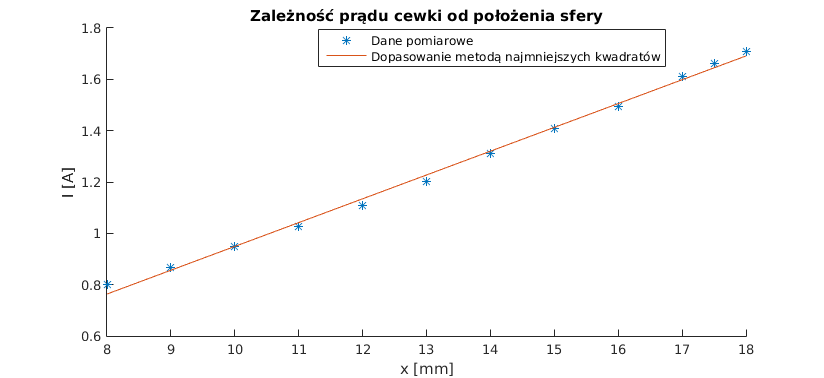
\includegraphics[scale=0.75]{img/identyfikacja_prad_cewki_od_polozenia.png}
\caption{Identyfikacja prądu cewki w funkcji położenia}
\label{rys:prad_od_polozenia}
\end{figure}

Dzięki identyfikacji możliwe było wyznaczenie parametrów prostej wspominanej we wzorze \ref{eq:Ix}, które niezbędne są do wyznaczenia wzoru na pochodną indukcyjności (wzór \ref{eq:L'}).

\begin{figure}[H]
\centering
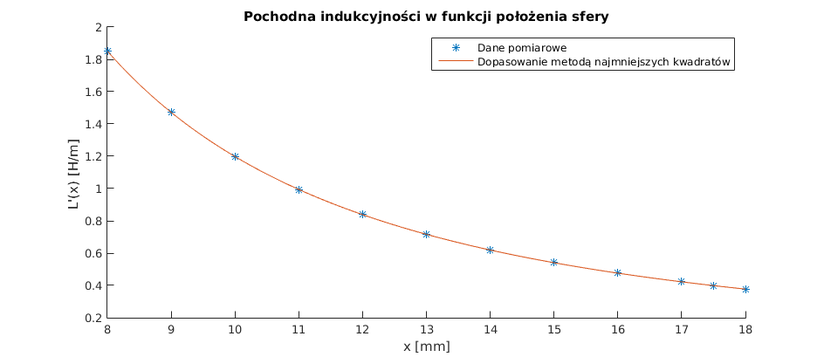
\includegraphics[scale=0.75]{img/identyfikacja_pochodna_indykcyjnosci_od_polozenia.png}
\caption{Identyfikacja pochodnej indukcyjności cewki w funkcji położenia}
\label{rys:pochodna_od_polozenia}
\end{figure}

Wszystkie wyznaczone parametry przedstawia tabela \ref{tab:parametry_ident}.

\begin{table}[H]
\begin{center}
  \begin{tabular}{| l | c | }
    \hline
    parametr 	& wartość \\ \hline
    $k$ & ... \\ \hline
    $T_{up}$ & $0.0245 s$  \\ \hline
	$T_{down}$ & $0.023 s$  \\ \hline
	$u_c$ & .. 	 \\ \hline
    $a$ 		  	& $0.0928$ \\ \hline
    $b$		  	& $0.0214$ \\ \hline
    kolejny parametr 			& 2.5 \\ \hline
    kolejny parametr 		& 0.52 \\
    \hline
  \end{tabular}
  \caption{Parametry wyznaczone w identyfikacji obiektu}
  \label{tab:parametry_ident}
\end{center}
\end{table}

\subsection{Weryfikacja modelu}

Porównanie obiektu i modelu 

[wykres stabilizacji PID obiektu]

[wykres porównania obiektu i modelu pod kontrolą PID]

%\begin{figure}[!htb]
%\centering
%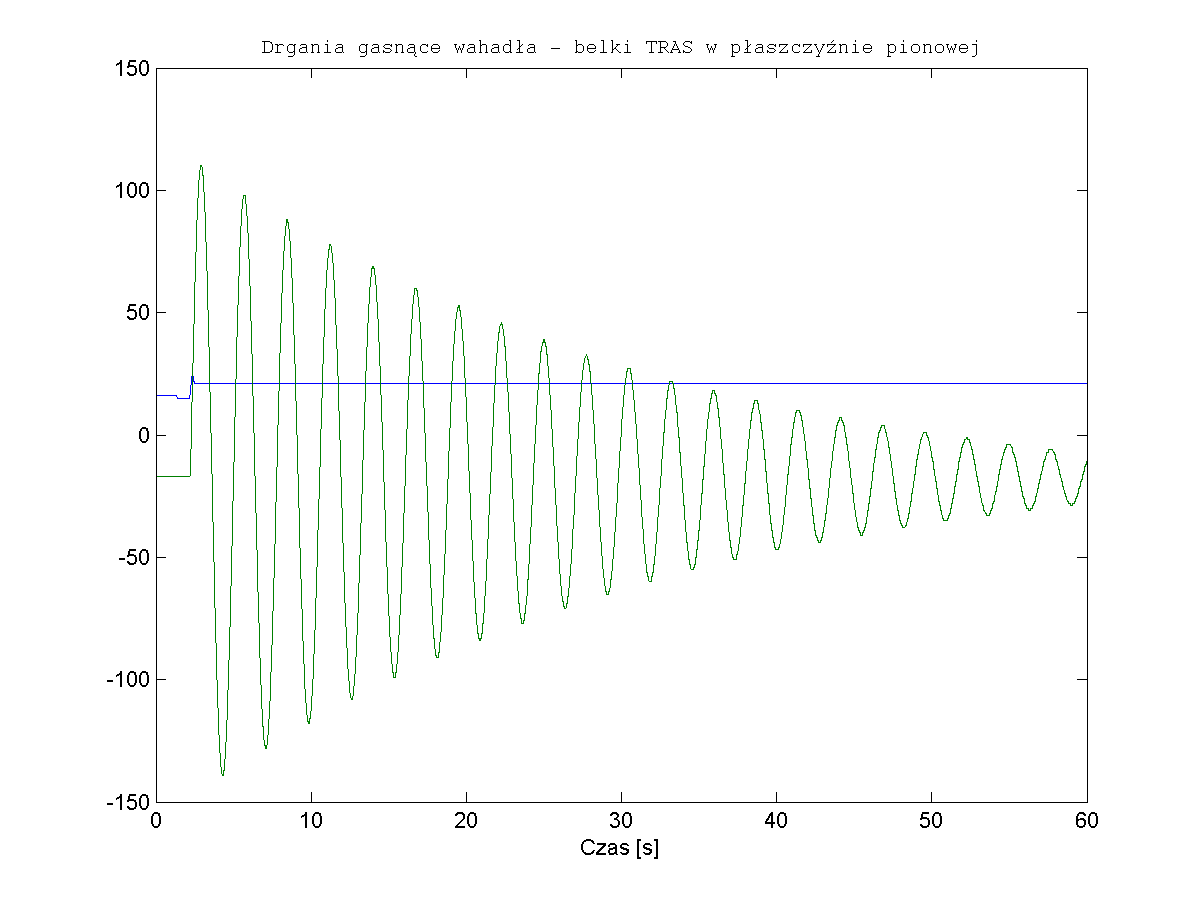
\includegraphics[scale=0.85]{img/gasnace.png}
%\caption{Identyfikacja oporów tarcia belki w płaszczyźnie pionowej}
%\label{rys:gasnace}
%\end{figure}


